\subsubsection{Enhancing Qthreads for ECP Science and Energy Impact} 


\paragraph{Overview} 

``Enhancing Qthreads for ECP Science and Energy Impact'' is a project that aims to improve the performance of applications that use multithreading with communication, e.g., MPI.  Most ECP applications are using this combination of programming models, with the Kokkos or RAJA performance portability libraries and/or the OpenMP API for multithreading.  This project supports the Kokkos ECP software project and OpenMP from the underlying runtime layer to deliver thread-scalable performance to those applications.  To that end, our projects is developing techniques to incorporate support for better network concurrency into the multithreading runtime system.

\paragraph{Key  Challenges}
Our project addresses the challenge of scalably coupling multithreaded parallelism on the many-core node with communication such as MPI, which has traditionally performed poorly in multithreaded mode.  The key challenge arises when multiple threads make communication calls, and those calls must be serviced by the MPI implementation and NIC.  Existing solutions, such as MPI\_THREAD\_MULTIPLE, are often plagued by synchronization overheads.  Even the best vendor MPI implementations incur high overheads when the number of threads exceeds the number of hardware contexts in the NIC. 
While current mechanisms are insufficient even for today's systems, emerging interconnect technologies expose even more network parallelism that must be exploited to maximize performance for Exascale.

\paragraph{Solution Strategy}

Unlike previous approaches, we attack the problem not only from the communication side (MPI), but with assistance from the multithreading runtime system.  Our work adds capabilities to enable the runtime system to identify and optimize for tasks that use communication, distinct from tasks that perform only local computation.  We use the Qthreads runtime~\cite{wheeler2008qthreads}, a scalable, event-driven library for node-level task parallelism, to implement our solution.  This work requires cooperation with a communication library that can scalably process communications operations coming from the runtime system.  For this purpose, we pair Qthreads with the new “FinePoints" library for threaded MPI execution developed in the OMPI-X ECP project.

Developed at Sandia Labs since 2007, Qthreads serves as a back-end for Kokkos and the Cray Chapel language, as well as providing a portable native C API. Complementary to the current ECP project focusing on the coupling of the runtime with communication, development of Qthreads core capabilities is part of the NNSA ASC system software portfolio and has also been part of sponsored vendor collaborations and LDRD projects.  In addition, the techniques developed in this project will be the subject of tech transfer efforts to OpenMP and MPI.  The project technical lead is chair of the OpenMP Subcommittee on Task Parallelism, and one of the other technical experts on the project is a key contributor to the MPI Forum and the OMPI-X ECP project that is enhancing the open-source Open MPI implementation of MPI for exascale.  We are leveraging the work of that project, and synergies between Qthreads and the OpenMP and Kokkos tasking models.


\paragraph{Recent Progress}

Most recently, we added the optional network task annotation to task definitions in Qthreads, allowing the identification of communication tasks to the runtime system.  We also demonstrated successful coupling of Qthreads with the MPI FinePoints library.  FinePoints uses a partitioned buffer to collect the contributions of the various tasks executing on the runtime’s threads.  Using only atomics rather than heavyweight locks keeps overhead costs low compared to existing methods like MPI\_THREAD\_MULTIPE, and unlike the Endpoints proposal, the MPI rank space does not expand with the use of more threads.  We ported FinePoints benchmark code to use Qthreads as the multithreading library instead of OpenMP and compared to the performance of the two configurations, shown in Figure~\ref{fig:qthreads-finepoints-graph}. The observed equivalence in performance justifies our use of Qthreads as a proxy for OpenMP, wherein Qthreads can be used for ease of rapid protoyping of new capabilities with eventual tech transfer back to OpenMP.  These results also serve as baselines to measure the performance of our further optimizations against.  Finally, we made an initial port of the miniGhost stencil mini-app to use FinePoints with Qthreads to confirm portability beyond benchmarks.  Tuning of that mini-app is currently work in progress.

\begin{figure}[htb]
	\centering
	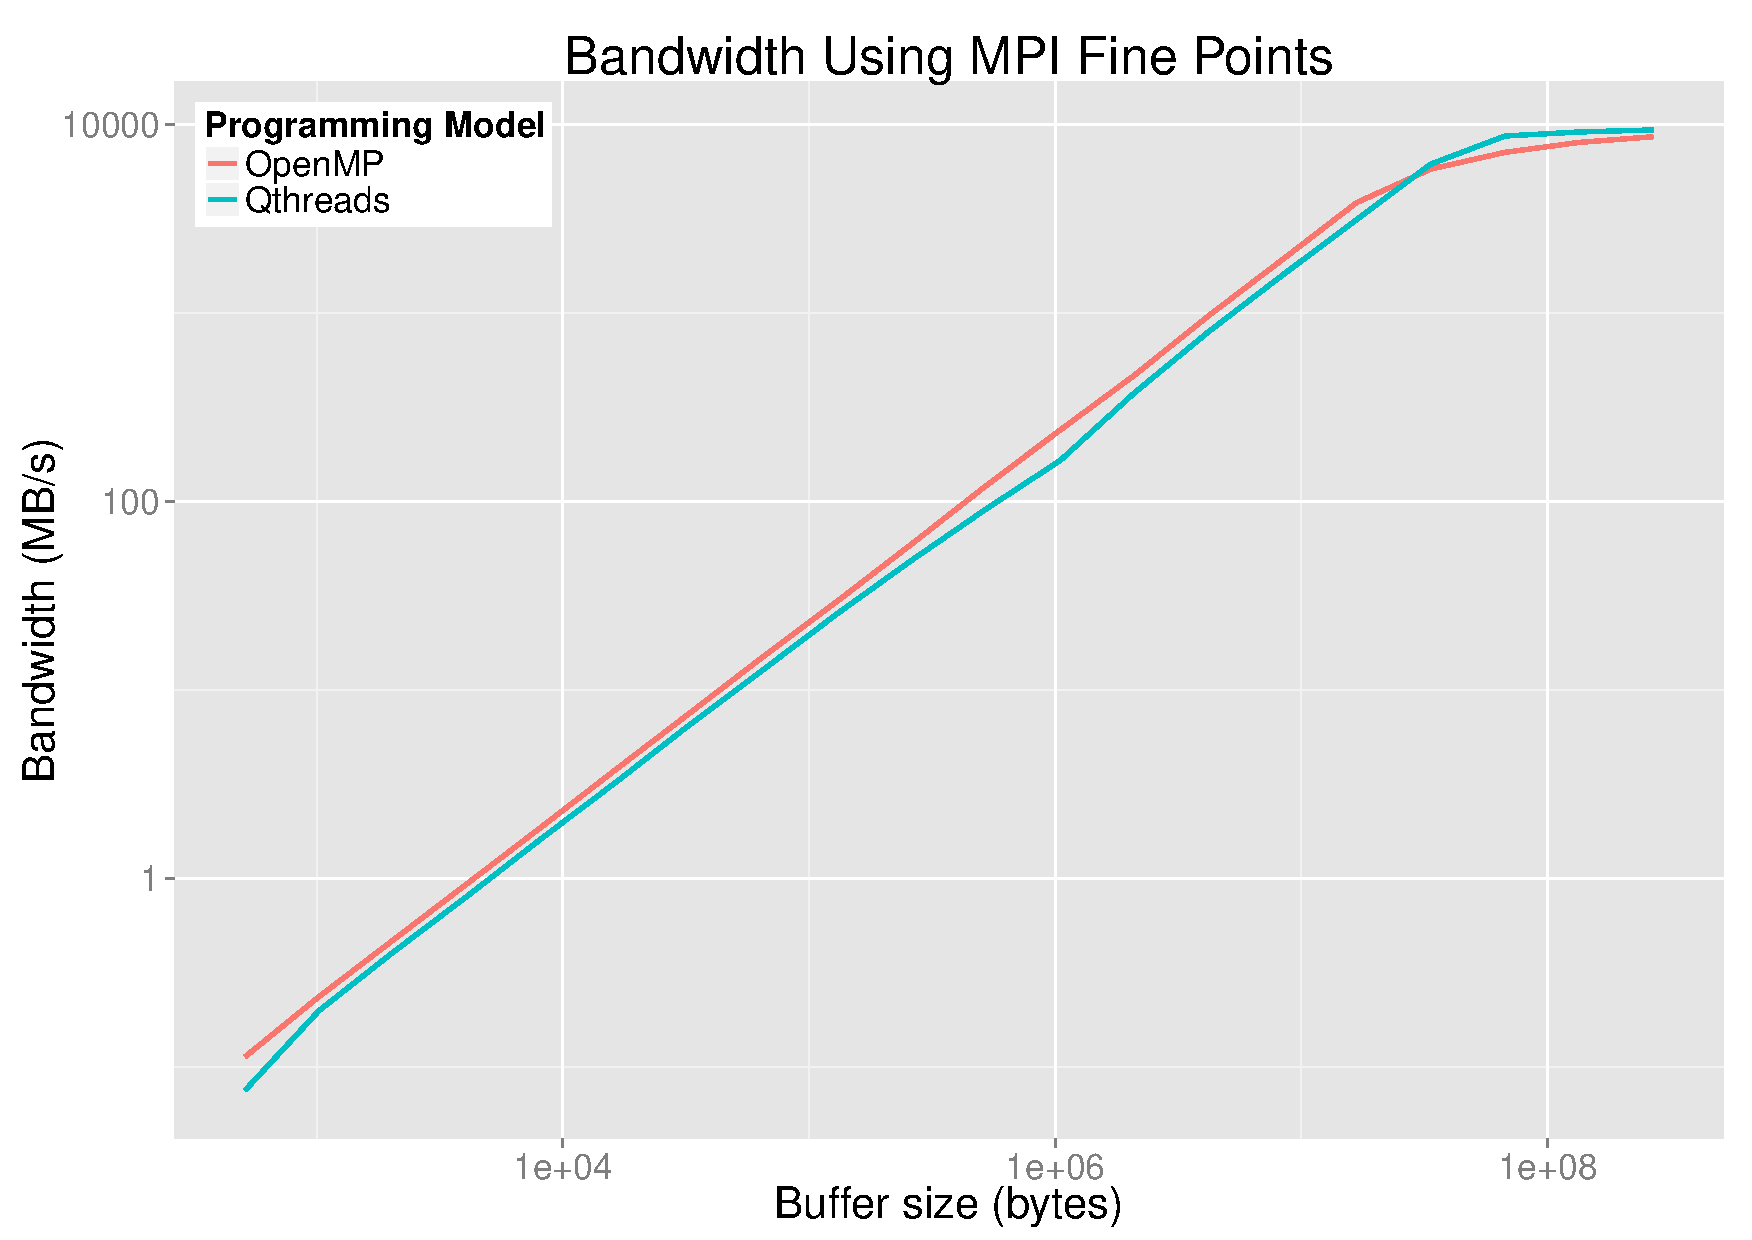
\includegraphics[width=6in]{projects/2.3.1-PMR/2.3.1.15-Qthreads/FinePointsBW-QtOmp.pdf}
	\caption{\label{fig:qthreads-finepoints-graph}This graph shows the performance of Qthreads and OpenMP paired with the FinePoints library for multithreaded MPI.  The x-axis varies the buffer sizes transferred in each experiment in the series, and the y-axis shows the network bandwidth achieved.  The similar performance of Qthreads and OpenMP justifies use of the former as a suitable proxy for the latter, with the advantage of flexibility for rapid prototyping of new runtime system techniques.}
\end{figure}


\paragraph{Next Steps}

We will investigate several possible optimizations, either in terms of Qthreads runtime improvements alone, or in conjunction with the OpenMPI implementation in which Finepoints is natively available as an extension:

\begin{itemize}
\item Enabling the swapping of schedulers in the Qthreads runtime at execution time in response to the tasks set observed.  (Currently the scheduler must be selected at configure time, so we would progress from there to selection at the start of an execution, and finally to a dynamic selection during the execution.)
\item To better enable the coordination of Qthreads and OpenMPI, add Qthreads as an MPI threading model instead of the default pthreads. (This requires modifying OpenMPI's “opal” subsystem to use a new threading mechanism.)
\item To explore this scheduling infrastructure, implement novel scheduling points (e.g. synchronization points in critical regions) allowing contended OpenMPI synchronization areas to schedule Qthreads events and vice versa.
\item With hierarchical and differential scheduling infrastructure in place, seek to design scheduling policies which optimize the interaction between composed runtimes.
\end{itemize}

We anticipate that due to technical and logistical constraints, only a subset of these tasks may be possible, but there will be value in at least attempting them and documenting our findings.  We feel confident that through this work, significant strides will be made toward better coupling of threading and communication.

